%%%%%%%%%%%%%%%%%%%%%%%%%%%%%%%%%%%%%%%%%
% Jacobs Landscape Poster
% LaTeX Template
% Version 1.0 (29/03/13)
%
% Created by:
% Computational Physics and Biophysics Group, Jacobs University
% https://teamwork.jacobs-university.de:8443/confluence/display/CoPandBiG/LaTeX+Poster
% 
% Further modified by:
% Nathaniel Johnston (nathaniel@njohnston.ca)
%
% This template has been downloaded from:
% http://www.LaTeXTemplates.com
%
% License:
% CC BY-NC-SA 3.0 (http://creativecommons.org/licenses/by-nc-sa/3.0/)
%
%%%%%%%%%%%%%%%%%%%%%%%%%%%%%%%%%%%%%%%%%

%----------------------------------------------------------------------------------------
%	PACKAGES AND OTHER DOCUMENT CONFIGURATIONS
%----------------------------------------------------------------------------------------

\documentclass[final]{beamer}

\usepackage[scale=1.24]{beamerposter} % Use the beamerposter package for laying out the poster

\usetheme{confposter} % Use the confposter theme supplied with this template

\setbeamercolor{block title}{fg=ngreen,bg=white} % Colors of the block titles
\setbeamercolor{block body}{fg=black,bg=white} % Colors of the body of blocks
\setbeamercolor{block alerted title}{fg=white,bg=dblue!70} % Colors of the highlighted block titles
\setbeamercolor{block alerted body}{fg=black,bg=dblue!10} % Colors of the body of highlighted blocks
% Many more colors are available for use in beamerthemeconfposter.sty

%-----------------------------------------------------------
% Define the column widths and overall poster size
% To set effective sepwid, onecolwid and twocolwid values, first choose how many columns you want and how much separation you want between columns
% In this template, the separation width chosen is 0.024 of the paper width and a 4-column layout
% onecolwid should therefore be (1-(# of columns+1)*sepwid)/# of columns e.g. (1-(4+1)*0.024)/4 = 0.22
% Set twocolwid to be (2*onecolwid)+sepwid = 0.464
% Set threecolwid to be (3*onecolwid)+2*sepwid = 0.708

\newlength{\sepwid}
\newlength{\onecolwid}
\newlength{\twocolwid}
\newlength{\threecolwid}
\setlength{\paperwidth}{48in} % A0 width: 46.8in
\setlength{\paperheight}{36in} % A0 height: 33.1in
\setlength{\sepwid}{0.024\paperwidth} % Separation width (white space) between columns
\setlength{\onecolwid}{0.22\paperwidth} % Width of one column
\setlength{\twocolwid}{0.464\paperwidth} % Width of two columns
\setlength{\threecolwid}{0.708\paperwidth} % Width of three columns
\setlength{\topmargin}{-0.5in} % Reduce the top margin size
%-----------------------------------------------------------

\usepackage{graphicx}  % Required for including images

\usepackage{booktabs} % Top and bottom rules for tables

%----------------------------------------------------------------------------------------
%	TITLE SECTION 
%----------------------------------------------------------------------------------------

\title{\emph{Middlemarch}: Critical Histories} % Poster title

\author{Jonathan Reeve, Sierra Eckert, Milan Terlunen} % Author(s)

\institute{Department of English and Comparative Literature, Columbia University} % Institution(s)

%----------------------------------------------------------------------------------------

\begin{document}

\addtobeamertemplate{block end}{}{\vspace*{2ex}} % White space under blocks
\addtobeamertemplate{block alerted end}{}{\vspace*{2ex}} % White space under highlighted (alert) blocks

\setlength{\belowcaptionskip}{2ex} % White space under figures
\setlength\belowdisplayshortskip{2ex} % White space under equations

\begin{frame}[t] % The whole poster is enclosed in one beamer frame

\begin{columns}[t] % The whole poster consists of three major columns, the second of which is split into two columns twice - the [t] option aligns each column's content to the top

\begin{column}{\sepwid}\end{column} % Empty spacer column

\begin{column}{\onecolwid} % The first column

%----------------------------------------------------------------------------------------
%	OBJECTIVES
%----------------------------------------------------------------------------------------

\begin{alertblock}{Objectives}

Lorem ipsum dolor sit amet, consectetur, nunc tellus pulvinar tortor, commodo eleifend risus arcu sed odio:
\begin{itemize}
\item Mollis dignissim, magna augue tincidunt dolor, interdum vestibulum urna
\item Sed aliquet luctus lectus, eget aliquet leo ullamcorper consequat. Vivamus eros sem, iaculis ut euismod non, sollicitudin vel orci.
\item Nascetur ridiculus mus.  
\item Euismod non erat. Nam ultricies pellentesque nunc, ultrices volutpat nisl ultrices a.
\end{itemize}

\end{alertblock}

%----------------------------------------------------------------------------------------
%	INTRODUCTION
%----------------------------------------------------------------------------------------

\begin{block}{Introduction}

Using 




\end{block}

%------------------------------------------------


%----------------------------------------------------------------------------------------

\end{column} % End of the first column

\begin{column}{\sepwid}\end{column} % Empty spacer column

\begin{column}{\twocolwid} % Begin a column which is two columns wide (column 2)

\begin{columns}[t,totalwidth=\twocolwid] % Split up the two columns wide column

\begin{column}{\onecolwid}\vspace{-.6in} % The first column within column 2 (column 2.1)

%----------------------------------------------------------------------------------------
%	MATERIALS
%----------------------------------------------------------------------------------------

\begin{block}{Frequently Quoted Chapters}

\begin{figure}
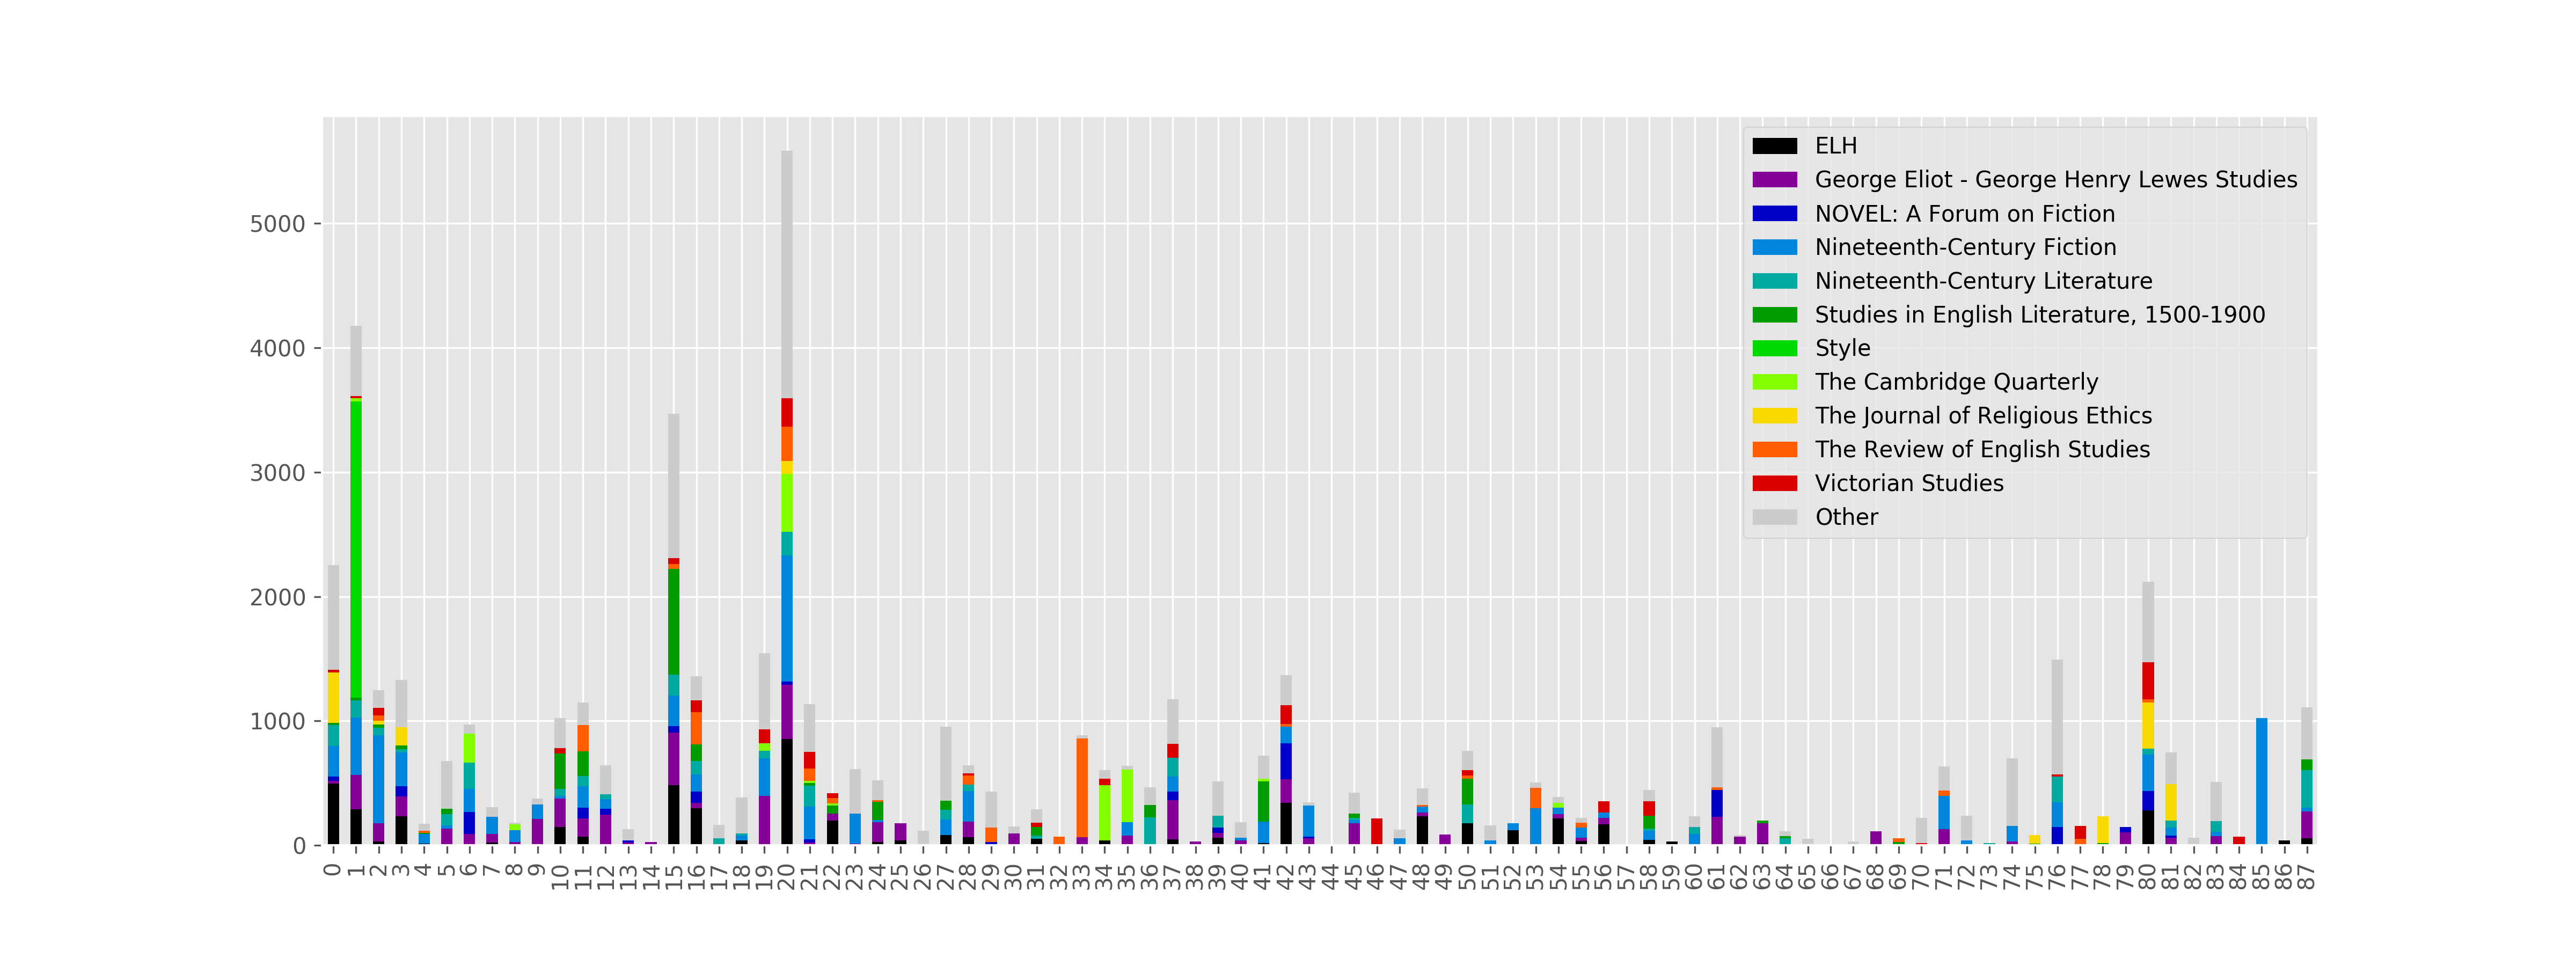
\includegraphics[width=0.8\linewidth]{synchronic-journals.png}
\caption{Quoted words by chapter, subdivided by journal.}
\end{figure}

\end{block}

%----------------------------------------------------------------------------------------

\end{column} % End of column 2.1

\begin{column}{\onecolwid}\vspace{-.6in} % The second column within column 2 (column 2.2)

%----------------------------------------------------------------------------------------
%	METHODS
%----------------------------------------------------------------------------------------

\begin{block}{Literary Critical Specialization}

Literary critics writing in the specialist journal \emph{George Eliot / George Henry Lewes Studies} quote different passages from their counterparts publishing in more generalist journals. A positive score here indicates a chapter is quoted more by specialists:  

\begin{figure}
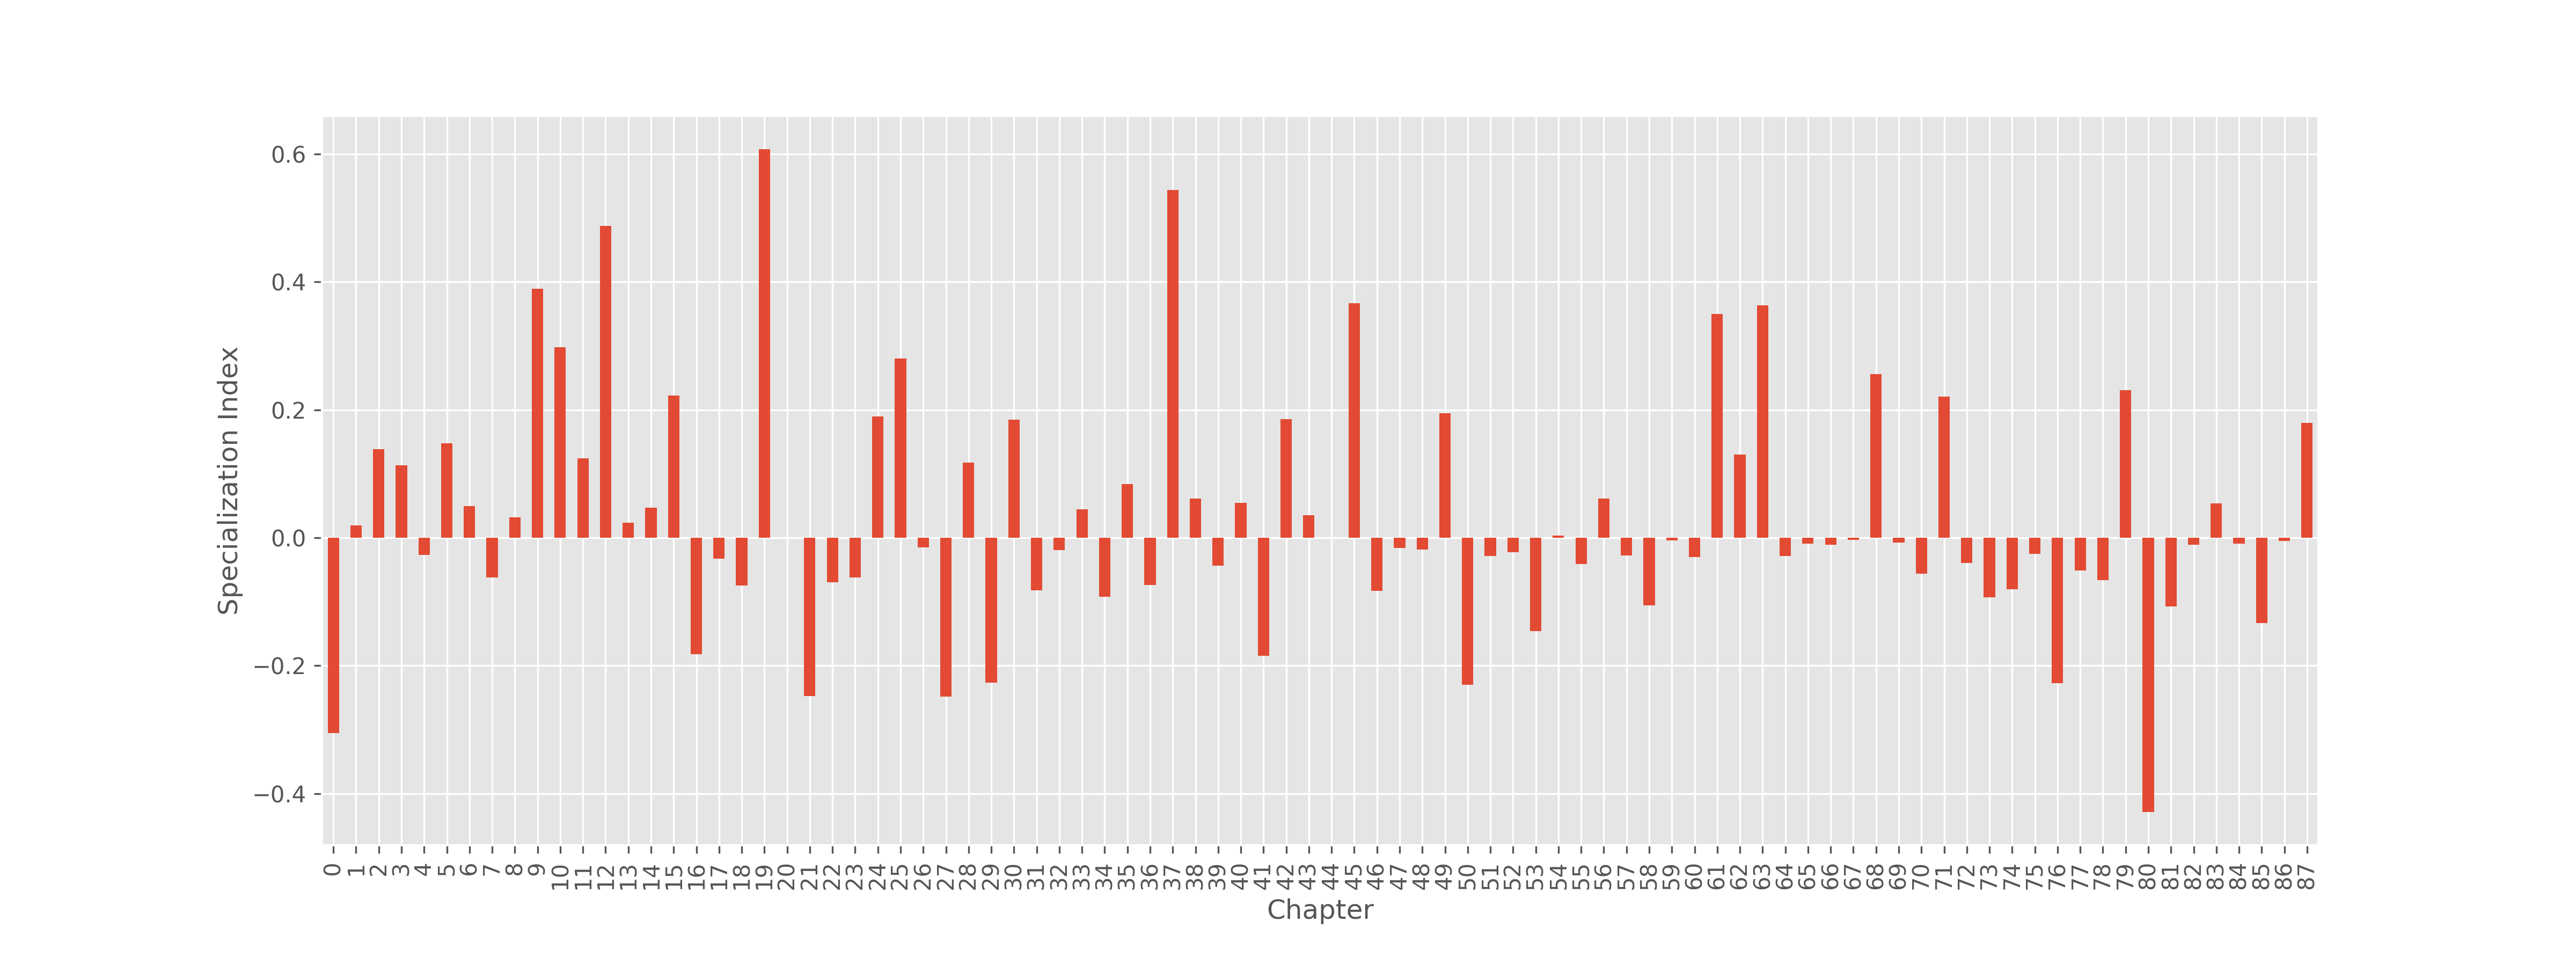
\includegraphics[width=0.8\linewidth]{specialization.png}
\caption{Difference in quotations between specialists and non-specialists.}
\end{figure}


\end{block}

%----------------------------------------------------------------------------------------

\end{column} % End of column 2.2

\end{columns} % End of the split of column 2 - any content after this will now take up 2 columns width

%----------------------------------------------------------------------------------------
%	IMPORTANT RESULT
%----------------------------------------------------------------------------------------

\begin{alertblock}{Shifts in Critical Attention over Time}

Viewed diachronically, trends arise in critical quotations of the novel. Critics' favorite chapters to excerpt shift from Chapter 81 in the 1950s to Chapter 20 in the 60s-70s, and to Chapter 15 in the 80s-90s. 

\begin{figure}
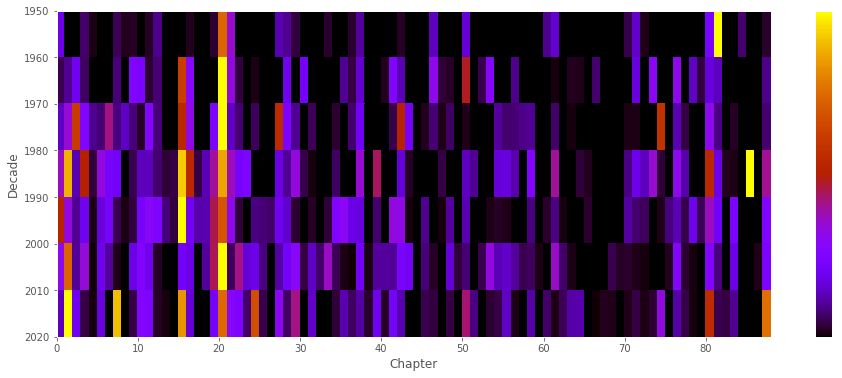
\includegraphics[width=0.8\linewidth]{diachronic.png}
\caption{Figure caption}
\end{figure}

\end{alertblock} 

%----------------------------------------------------------------------------------------

\begin{columns}[t,totalwidth=\twocolwid] % Split up the two columns wide column again

\begin{column}{\onecolwid} % The first column within column 2 (column 2.1)

%----------------------------------------------------------------------------------------
%	MATHEMATICAL SECTION
%----------------------------------------------------------------------------------------

\begin{block}{Mathematical Section}

Nam quis odio enim, in molestie libero. Vivamus cursus mi at nulla elementum sollicitudin. Nam quis odio enim, in molestie libero. Vivamus cursus mi at nulla elementum sollicitudin.
  
\begin{equation}
E = mc^{2}
\label{eqn:Einstein}
\end{equation}

Nam quis odio enim, in molestie libero. Vivamus cursus mi at nulla elementum sollicitudin. Nam quis odio enim, in molestie libero. Vivamus cursus mi at nulla elementum sollicitudin.

\begin{equation}
\cos^3 \theta =\frac{1}{4}\cos\theta+\frac{3}{4}\cos 3\theta
\label{eq:refname}
\end{equation}

Nam quis odio enim, in molestie libero. Vivamus cursus mi at nulla elementum sollicitudin. Nam quis odio enim, in molestie libero. Vivamus cursus mi at nulla elementum sollicitudin.

\begin{equation}
\kappa =\frac{\xi}{E_{\mathrm{max}}} %\mathbb{ZNR}
\end{equation}

\end{block}

%----------------------------------------------------------------------------------------

\end{column} % End of column 2.1

\begin{column}{\onecolwid} % The second column within column 2 (column 2.2)

%----------------------------------------------------------------------------------------
%	RESULTS
%----------------------------------------------------------------------------------------

\begin{block}{Results}

\begin{figure}

\includegraphics[width=0.8\linewidth]{placeholder.jpg}
\caption{Figure caption}
\end{figure}

Nunc tempus venenatis facilisis. Curabitur suscipit consequat eros non porttitor. Sed a massa dolor, id ornare enim:


\end{block}

%----------------------------------------------------------------------------------------

\end{column} % End of column 2.2

\end{columns} % End of the split of column 2

\end{column} % End of the second column

\begin{column}{\sepwid}\end{column} % Empty spacer column

\begin{column}{\onecolwid} % The third column

%----------------------------------------------------------------------------------------
%	CONCLUSION
%----------------------------------------------------------------------------------------

\begin{block}{Properties of Quotations}

Figure 5 shows characteristic parts of speech of quotations (positive), and non-quotations (negative). 

\begin{figure}
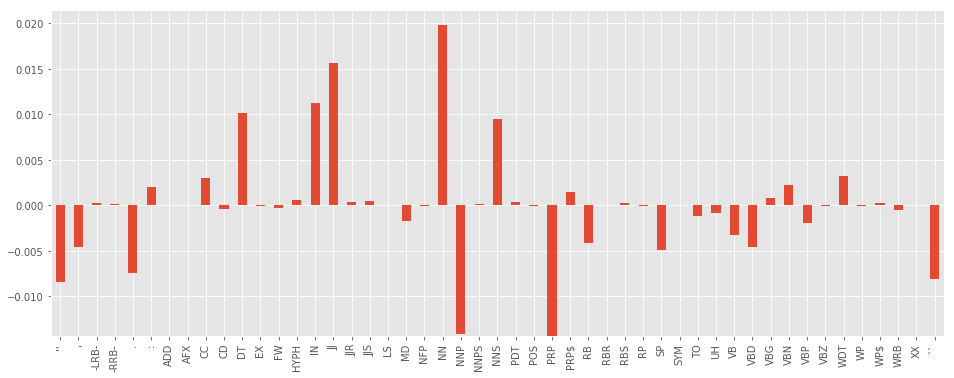
\includegraphics[width=0.8\linewidth]{pos-tags.png}
\caption{Distinctive parts of speech of quotations}
\end{figure}

Table 1 shows most distinctive words of non-quotes (negative, above), and quotes (positive, below): 

\begin{table}
\vspace{2ex}
\begin{tabular}{l l}
\toprule
\textbf{Word} & \textbf{Freq. Diff.} \\
\midrule
say           &  -0.006397 \\
lydgate       &  -0.004499 \\
mr.           &  -0.003395 \\
bulstrode     &  -0.002948 \\
fred          &  -0.002781 \\
rosamond      &  -0.002616 \\
\midrule
eye          &   0.001024 \\
live         &   0.001042 \\
consciousness &   0.001054 \\
great        &   0.001080 \\
new          &   0.001134 \\
woman        &   0.001154 \\
world        &   0.001883 \\
light        &   0.002183 \\
life         &   0.002417 \\
\bottomrule
\end{tabular}
\caption{(Non-)Distinctive words of quotations}
\end{table}

\end{block}

%----------------------------------------------------------------------------------------
%	ADDITIONAL INFORMATION
%----------------------------------------------------------------------------------------

\begin{block}{Links and Contacts}

\begin{itemize}
\item Project page: github.com/lit-mod-viz/middlemarch-critical-histories
\item Jonathan Reeve: jonathan.reeve@columbia.edu
\item Sierra Eckert: sierra.eckert@columbia.edu
\item Milan Terlunen: m.terlunen@columbia.edu 
\end{itemize}

\end{block}

%----------------------------------------------------------------------------------------

\end{column} % End of the third column

\end{columns} % End of all the columns in the poster

\end{frame} % End of the enclosing frame

\end{document}
